%% ----------------------------------------------------------------------
%% Esta es una plantilla para la clase de documento exam, en español
%% ----------------------------------------------------------------------
%% 2017 por Fausto M. Lagos S. <piratax007@protonmail.ch>
%% 
%% Este trabajo puede ser distribuido o modificado bajo los
%% términos y condiciones de la LaTeX Project Public License (LPPL) v1.3C, 
%% o cualquier versión posterior. La última versión de esta licencia
%% puede verse en:
%% http://www.latex-project.org/lppl.txt
%% 
%% Usted es libre de usarlo, modificarlo o distribuirlo siempre que se
%% respeten los términos de la licencia y se reconozca al autor original
%% ----------------------------------------------------------------------

%Preámbulo
\documentclass[10pt, legalpaper]{exam}
\usepackage[utf8]{inputenc}
\usepackage[spanish]{babel}
\usepackage[margin=.75in]{geometry}
\usepackage{amsmath,amssymb}
\usepackage{multicol}
\usepackage{graphicx}
\usepackage{tikz}

% Configuración del Encabezado
%\newcommand{\class}{Circuitos RLC}
\newcommand{\term}{Mayo Agosto 2024}
\newcommand{\examnum}{Segundo Parcial}
\newcommand{\examdate}{Fecha: 27 Julio }
\newcommand{\timelimit}{90 minutos}
\pagestyle{head}
\firstpageheader{Universidad Central del Este}{}{Escuale de Ingenieria Electromecanica }
\runningheader{\class}{\examnum\ - Page \thepage\ of \numpages}{\examdate}
\runningheadrule

% Configuración de la tabla de calificación
\pointpoints{punto}{puntos}
\hpword{Puntos:}
\vpword{Puntos}
\vtword{Total:}
\htword{Total}
\vsword{Resultado}
\hsword{Resultado:}
\vqword{Problema}
\hqword{Pregunta:}

\begin{document}
% Definición del Encabezado
\noindent
\begin{tabular*}{\textwidth}{l @{\extracolsep{\fill}} r @{\extracolsep{6pt}} l}
\textbf{\class} & \textbf{Nombre:} & \makebox[2.5in]{\hrulefill}\\
\textbf{\term} &&\\
\textbf{\examnum} & \textbf{Matricula:} & \makebox[2.5in]{\hrulefill}\\
\textbf{\examdate} &&\\
\textbf{Tiempo: \timelimit} & Profesor: & \makebox[2.5in]{\emph{Yeuris Adolfo Lopez Jaime, Msc.}}
\end{tabular*}\\
\rule[2ex]{\textwidth}{2pt}

% Bloque de instrucciones
\noindent
%Este examen contiene \numquestions \;planteamientos que corresponde a \numpoints \;puntos de la valoración final. Tenga presente que no esta autorizada la comunicación con sus compañeros, ni el uso de ayudas computacionales (calculadora, celular, etc) y que resolver el pliego a l\'apiz implica renunciar a cualquier reclamación después de entregados los resultados.

% Tabla de calificaciones
\begin{center}
Tabla de calificación de uso exclusivo para el profesor. \\
\addpoints
% Puede presentar la tabla de calificación en orientación vertical [v] u horizontal [h]
\gradetable[h][questions]
\end{center}

% Preguntas de ejemplo.
\begin{questions}
\addpoints
\question[5]  Una aplicación de un circuito RC es el oscilador de relajación, como se muestra a continuación. El oscilador de relajación consta de una fuente de tensión, una resistencia, un condensador y una lámpara de neón. La lámpara de neón actúa como un circuito abierto (resistencia infinita) hasta que la diferencia de potencial a través de la lámpara de neón alcanza un voltaje específico. A ese voltaje, la lámpara actúa como un cortocircuito (resistencia cero), y el condensador se descarga a través de la lámpara de neón y produce luz. En el oscilador de relajación mostrado, la fuente de tensión carga el condensador hasta que la tensión a través del condensador es de 80 V. Cuando esto ocurre, el neón de la lámpara se rompe y permite que el condensador se descargue a través de la lámpara, produciendo un destello brillante. Después de que el condensador se descargue completamente a través de la lámpara de neón, comienza a cargarse de nuevo, y el proceso se repite. Suponiendo que el tiempo que tarda el condensador en descargarse es despreciable, ¿cuál es el intervalo de tiempo entre destellos?

	\begin{figure}[h]
	    \centering
	    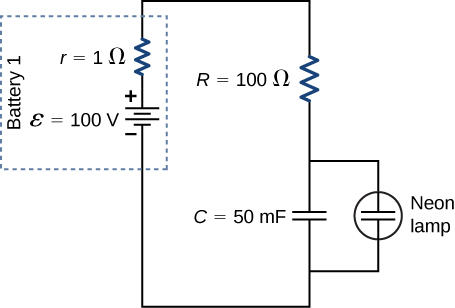
\includegraphics[width=0.5\linewidth]{CNX_UPhysics_27_05_Ex1_img.jpg}
	    \caption{Circuto de un oscilador de relajación}
	    \label{fig:enter-label}
	\end{figure}
\addpoints

\addpoints
\question[5] En un circuito RLC en serie con: L=5.0mH, C=6.0 $\mu$F, y  R=200 $\Omega$. (a) ¿Está el circuito subamortiguado, críticamente amortiguado o sobreamortiguado? (b) Si el circuito empieza a oscilar con una carga de 3,0×10-3C en el condensador, ¿cuánta energía se ha disipado en la resistencia cuando cesan las oscilaciones?

\addpoints
\question[5] Considere el circuito de la Figura 2. (a) ¿Cual es la constante de tiempo del circuito? (b) ¿Cual es la correinte inicial una vez el interruptor esta cerrado?. (c) ¿Que tanto tiempo pasa entre el isntante que el interruptor es cerrado y el tiempo que la corriente alcanza la mitad del valor de la corriente inicial?
	\begin{figure}[h]
	    \centering
	    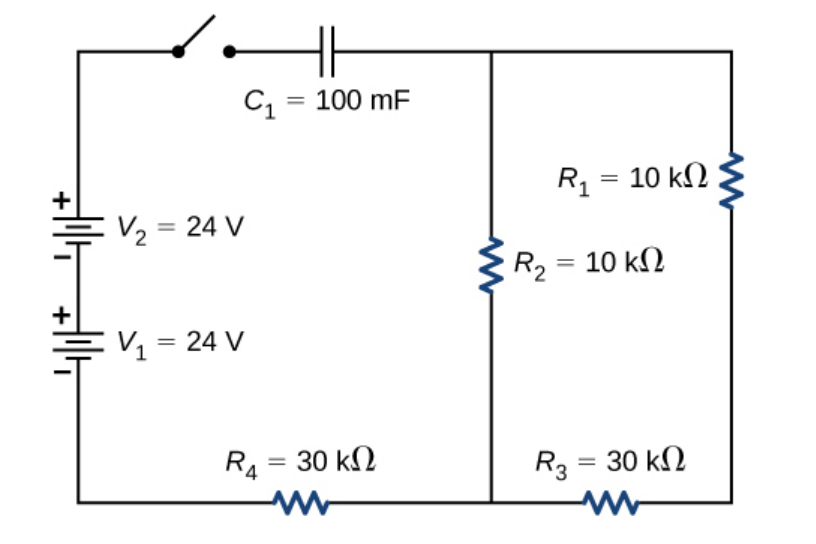
\includegraphics[width=0.8\linewidth]{Screenshot 2024-07-26 231805.png}
	    \caption{Circuito RC}
	    \label{fig:enter-label}
	\end{figure}

\addpoints
\question[5] En el circuito de la Figura 3, el interruptor ha estado cerrado durante mucho tiempo y en $t = 0$ cambia a la posicion 2. Obtenga $i(t)$ y $v(t)$ para $ t > 0$. Considera al capacitor inicialmente descargado. Diga si el sistema es subamortiguado, sobreamortigado o criticamente amortiado. Dibuje una grafica aproximada de la respuesta.
\begin{figure}[h]
    \centering
    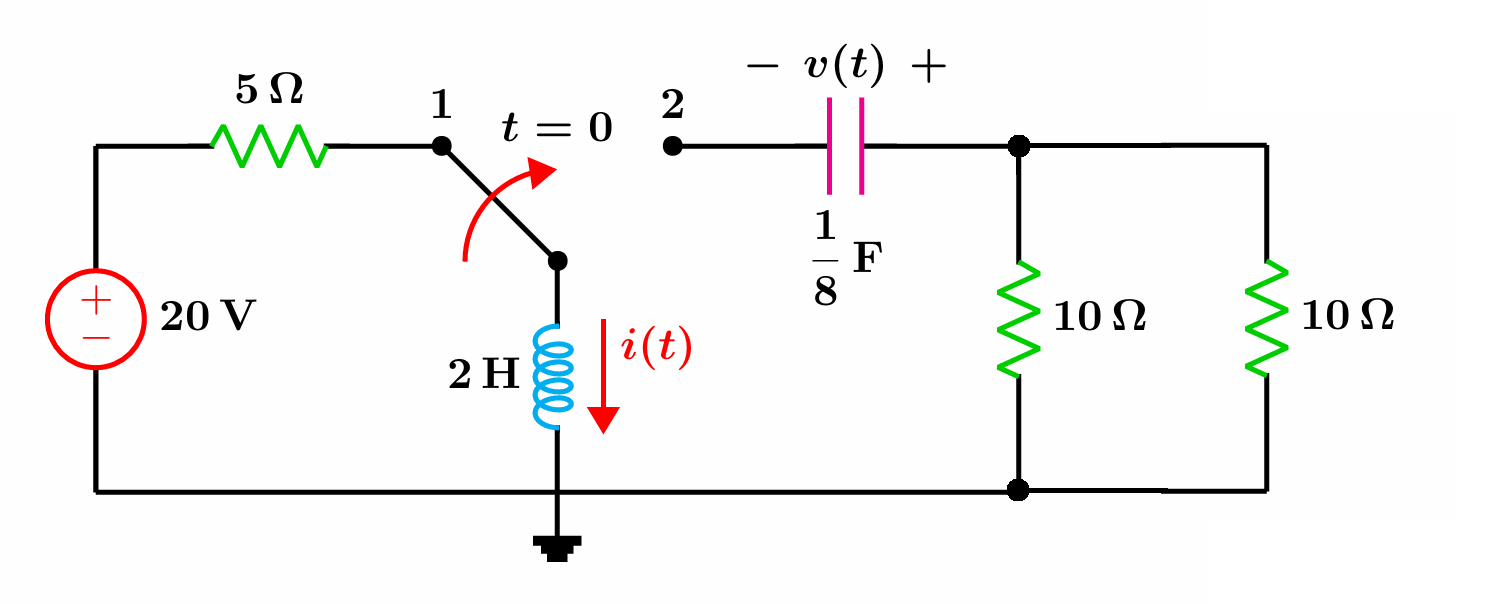
\includegraphics[width=0.7\linewidth]{Screenshot 2024-07-26 222326.png}
    \caption{Circuito RLC}
    \label{fig:enter-label}
\end{figure}
\question[5] Considere el circuito de la Figura 4. (a) ¿Cual es la corriente inicial en la resistencia $R_2$ cuando el interruptor esta cerrado? (b) ¿Cual es la correinte en la resistencia $R_2$ cuando el capacitor esta totalmente cargado, pasado mucho tiempo que el interruptor esta cerrado? (c) ¿Que pasa si el interruptor es abierto luego que tiene un tiempo cerrado? (d) ¿Si el interruptor ha estado cerrado por un perido de tiempo suficiente para que el capacitor se cargue por completo, y el interruptor es abierto, que tiempo debe pasar para que el valor de la corriente en $R_1$ alcance la mitad de su valor?
\begin{figure}[h]
    \centering
    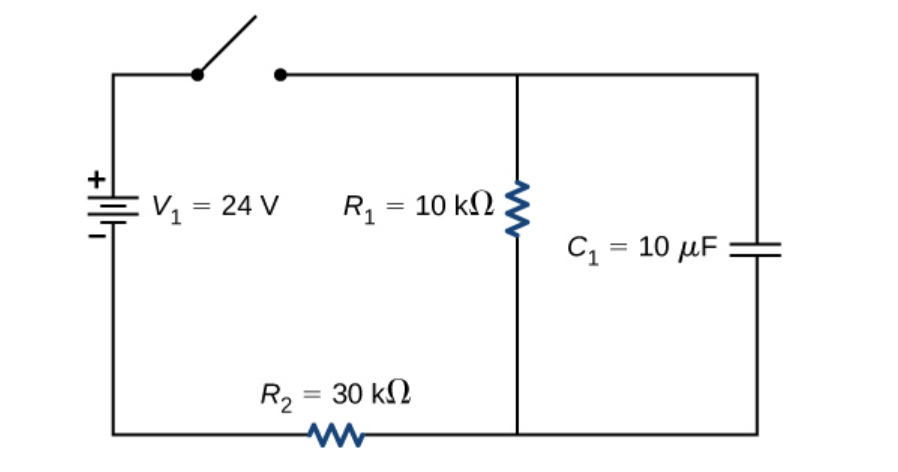
\includegraphics[width=0.8\linewidth]{Screenshot 2024-07-26 232957.png}
    \caption{Circuitor RC}
    \label{fig:enter-label}
\end{figure}
\question[5] Para un circuito RLC en serie con valores de  L = XH y C = $\frac{3}{X}$F, determine los valores de la resistencia que harian tener una respuesta sobreamrotiguada, subamortiguada y criticamente amrotiguada.

\end{questions}
\


\end{document}